\documentclass[11pt]{article}
\setlength{\parskip}{0.2cm}
\setlength{\parindent}{0cm}
\usepackage[hmargin=2.0cm,vmargin=2.3cm]{geometry}
\usepackage{url}
\usepackage{hyperref}
\usepackage{breakurl}
\usepackage{float}

% For footnotes
\usepackage{endnotes}
\let\footnote=\endnote

% To display two columns side-by-side.
\newcommand{\twofigure}[4]{
\begin{minipage}{0.45\textwidth}
    \centering
    \includegraphics[scale=0.35]{#1}
    \caption{#2}
\end{minipage}
\begin{minipage}{0.45\textwidth}
    \centering
    \includegraphics[scale=0.35]{#3}
    \caption{#4}
\end{minipage}
}

\ifx\pdftexversion\undefined
\usepackage[dvips]{graphicx}
\else
\usepackage[pdftex]{graphicx}
\DeclareGraphicsRule{*}{mps}{*}{}
\fi

\begin{document}

\title{Web Apps Project Report}

\author{Harry Lachenmayer, Artur Spychaj, Alex Rozanski and Thomas Rooney}

\date{\today}         % inserts today's date

\maketitle            % generates the title from the data above

\section {Introduction}

Our web app is a tool to help Imperial students find out about events happening on campus.

Most people currently find out about events through noticeboards and mailing lists. The problem with these is that there is no easy, centralised way of finding out what is happening on campus. A big problem with the noticeboards is that a lot of the posters are outdated, and often irrelevant. It is also difficult to find out which mailing lists to subscribe to to find interesting events. Additionally, the Imperial College home page and the Union website have event calendars. An `Imperial Mobile' application exists, which pulls data from the Imperial and Union sites, but we found that very few people use this, as it is complicated and slow.

\subsection{Requirements}

Our main aim is to bring all these disparate sources together and make a simple, `one-stop' solution to find interesting events.

To achieve this, we identified three main requirements for the design of the app. The app should be:

\begin{itemize}
    \item \textbf{Simple} \\[0.5em] Users should immediately see relevant and interesting events. There should be no barrier of entry, such as registering or logging in, for most activities in the app.

    \item \textbf{Relevant} \\[0.5em] There are many different kinds of events happening on campus. Many of these are interesting to only a small subset of the college population. Users should be able to focus on events that are relevant to their interests.

    \item \textbf{Up-to-date} \\[0.5em] Advertising events on campus should be as easy as entering the event details once. Users should be able to stay up to date on the latest events without any effort.

\end{itemize}

We wanted to make the user interaction with the system as easy as possible. To that end, we identified the following priorities:

\begin{itemize}
\item Authenticate with the college systems: no need to register a separate account. We consider this incredibly important because to attract a user base from nothing we need to make the barrier to entry as low as possible.

\item Provide automatic access to \textit{at least} the feeds that we already have access to, such as the Imperial College Union `What's On' calendar. We wanted to provide value without user interaction, so that it can be used immediately as an information source.

\item Allow users to add events. While the website is intended to be a good source of information, the hope is that it could become the preferred platform for organising events by Imperial students and committees.
\end{itemize}

\subsection {Target Audience}

The first stage in our project was to define our target user(s). We decided on limiting our users to members of the College, but we split these into the following sub-groups, and for each we created user stories describing their key characteristics:

\subsubsection{Undergraduate}
Harry is an undergraduate at Imperial College. He is a member of a few societies, but does not hold any executive committee positions. He likes going to events organised by the societies he is a member of, and other Union-organised events. He loves free stuff, especially free food, but usually finds out about events that give away free stuff far too late. He has a lot of friends that are really involved in societies, and is often invited to events by them through Facebook and society email lists. He is looking for an internship this summer. He was in halls in first year and knows a lot of people from there that he rarely sees anymore.

\subsubsection{Postgraduate}
Adam is currently doing his PhD in bio-chemistry. He attends many evening lectures relating to research topics that he is interested in. He is also a fan of classical music and likes to attend lunchtime concerts. He is an avid snowboarder and surfer and regularly goes to snow domes with the ski society and week-long trips with the surfing society. He has recently become interested in starting a company, and goes to business school events to meet fellow entrepreneurs. He is not particularly interested in any Union events.

\subsubsection{Event Organisers}
Lizzy is really involved in Union activities. She writes for Felix, and is the president of a mid-sized society. She is also the social secretary of another large society. She uses Facebook to invite people to nights out organised by these societies, and regularly uses the society email lists to announce society meetings and smaller events. She currently uses Google Docs spreadsheets to manage attendance to these smaller events.
\section {Project Management}

\subsection {Group Structure}

We split our group into two teams: one consisting of Alex and Harry, who worked on the client side, and the other consisting of Tom and Artur, who worked on the server-side implementation. As discussed below, we adhered to Agile development practices, whilst operating as a leaderless group. We found this process happened naturally, with all of us been able to contribute and integrate our various ideas into a single product. We believe that working in this manner was made possible by knowing each other and our differing skills well, and removed the overhead that having a formal group leader or facilitator role can add.

\subsection {Design Processes}

Throughout the project, we took both an agile approach by continuously iterating on ideas, but we also planned heavily up-front before we started development to establish our target users and the design of our app. This was very important to us as the cost and amount of work required to make changes grows exponentially the later on in the development of the product they are made.

We started out by creating a business model canvas, which allowed us to think about aspects to the project such as the target audience and the viability of our app as a product. We also devised user stories for our target users to get a better understanding of the problems they face and how our project would address these.

Still before we'd even written a single line of code, we designed the user interaction and a rough outline for the user interface. We iterated on designs and mockups until we had a workflow and experience that we were happy with.

At this point, we decided on which technologies to use to build our project with for both the front-end and back-ends. We then started to implement features and iterated on them until we were happy with the result. Although we split ourselves into two teams (for the front-end and back-end), we made sure to constantly integrate both parts to find and fix issues as early as possible during the development process.

\subsection {Collaborative Tools}
\subsubsection {GitHub Wiki}
We used the GitHub Wiki as a place to document areas of the project as we implemented them. For example, both the client-side and server-side teams each documented the process involved in setting up their respective system, so that other group could always run the entire system to test the part they were working on with the other components.

We also created Wiki entries for the REST API specification as it was being implemented server-side. This meant that the client-side group could interact with it and start testing calls to it as early as possible.
\subsubsection {Trello}

Trello\footnote{\url{http://trello.com}} is an organisational and management web application produced by FogCreek. It provides a collection a lists of items, each of which can be thought of as a list of small items (which can be expanded in more detail underneath).

\begin{figure}[H]
\centering
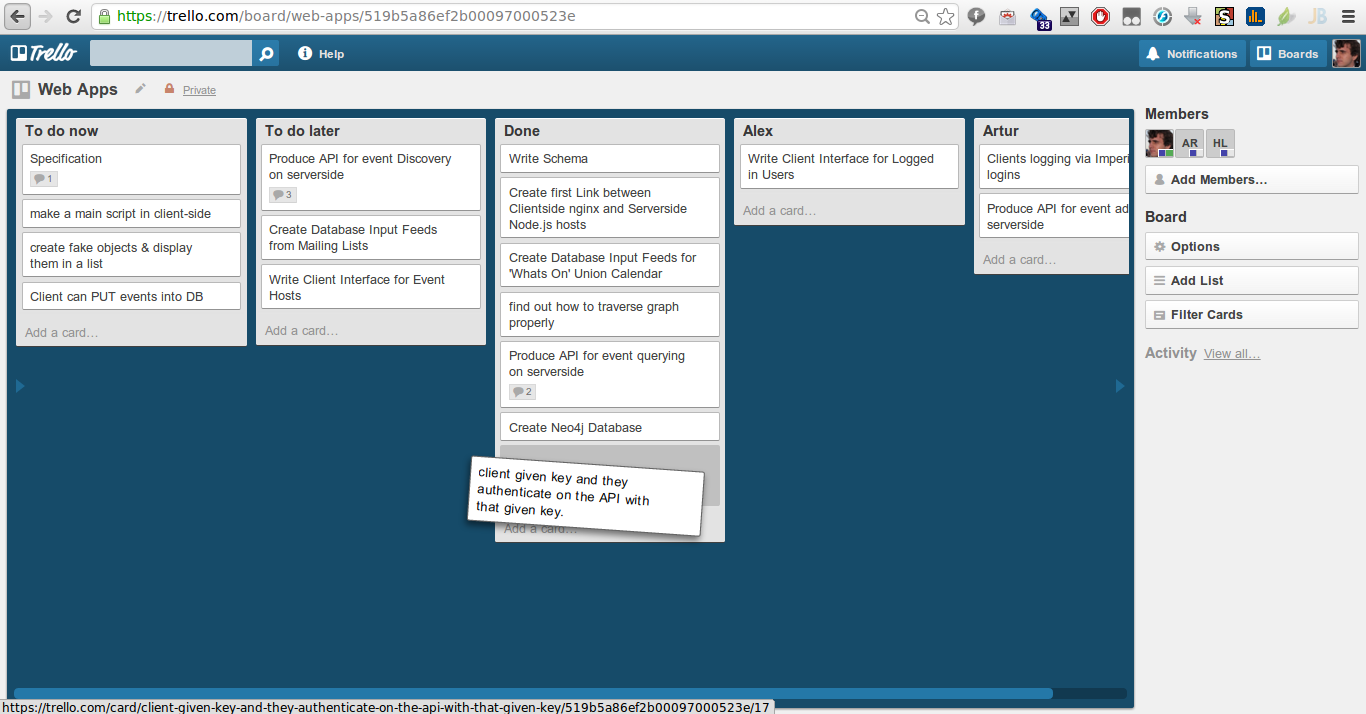
\includegraphics[scale=0.35]{images/trello.png}
\caption{\label{fig:trello} Trello - Collaborative Organizational Tool}
\end{figure}
In following the Agile development methodology of an iterative development, we used Trello to define new tasks during our group meetings. In doing this, we could effectively ensure that there was fair and consistent contribution from all members by assigning each task to somebody on Trello. This also allowed us all to keep track of where we were in the project, an maintain a consistent list of tasks we needed to do, minimizing the `what now?' time.

\subsection{Backup Systems}
We used git as our version control system for the project, and hosted the repository privately on GitHub. Although git is a decentralised version control system, having the project hosted on GitHub, as well as the local clones we all had on our machines meant we had enough redundancy that if one of our copies was accidentally deleted it would have little effect on our project (we also all regularly committed our changes and pushed them upstream).

What's more, we built the project so that it was very easy to get up-and-running on a server from a fresh clone of the repository. As we were using three servers (the front-end server, the back-end server and the database server) we wrote scripts which would start, stop and restart all the servers with one command. This also meant that if our VM server given to us by CSG were to fail, even though it was not backed up itself, we could very quickly get the servers up and running again.

\section{The System}

When a user first opens the app, they see a list of future events starting from today. The user can tap/click on any event to see further details about that event.

The user can also browse a list of tags, and order them alphabetically, or by their popularity (how many events are categorised under each).


\begin{figure}[H]
\twofigure{images/event-list.png}{The main event list.}{images/event-detail.png}{The details for a single event.}
\\[2em]
\end{figure}
\begin{figure}[H]
\twofigure{images/tag-list.png}{The list of tags a user can subscribe to.}{images/login.png}{The login screen.}
\end{figure}
\begin{figure}[H]
\begin{minipage}{0.45\textwidth}
    \centering
    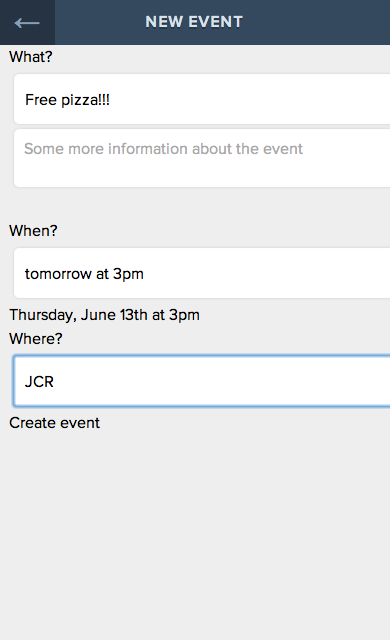
\includegraphics[scale=0.35]{images/new-event.png}
    \caption{The UI for creating a new event}
\end{minipage}
\end{figure}


\section {System Implementation}

In this project we wanted to experiment with some new technologies which are only starting to become widely used. We focus here on our implementation choices and some of the reasoning behind these.

\subsection{CoffeeScript}

We chose to develop our application using CoffeeScript, a programming language with a clean and elegant syntax which compiles down to JavaScript. We realised that building a rich web application would involve writing a lot of client-side JavaScript code. JavaScript however has many quirks, many of which are nicely dealt with in CoffeeScript. As one of the team members already had considerable experience using CoffeeScript prior to the project, it was an obvious choice for the client-side application code. CoffeeScript's main syntactical feature is its use of significant whitespace, similar to Python.

\subsection {Front End}

Our application relies heavily on client-side JavaScript running in the browser to display the various views, using data loaded from the server via its REST interface.
We are using a popular JavaScript MVC-like library called Backbone. This library provides us with ``hassle-free" model synchronisation with the server and useful ways of dealing with UI changes in our view code. It is a small library, and leaves a lot of freedom for implementation details. For example, it doesn't prescribe any particular HTML templating engine.

We are using a templating language called Jade, which uses significant whitespace to indicate nested tags, rather than opening/closing tags. This results in much smaller and more understandable HTML templates. Our CSS styles are written in a language called Stylus, which again uses significant whitespace, and allows nesting of style rules.

In parts of the UI we are using a library called Bacon.js, which is a ``functional reactive programming" library. Functional reactive programming represents UI events as ``event streams". These streams are collections that can be manipulated using functional methods such as map, filter, etc. This allows for reasoning about UI state as it evolves over time. We are using to validate the data in one of our forms, ensuring that only valid data can be sent to the backend. More ``traditional" programming methods would probably have been easier to implement, but we believe that this is an exciting technology. It brings the benefits of functional programming to UI code, which is usually error-prone and difficult to test.

The front-end application is divided into logically separate components. Each view is a separate component, namely the events list, single event view, event creation view, login view and tag list view. Our data model is stored in the ``model" component. This contains definitions for the event and tag collections. In Backbone, each model is essentially just a definition of a server URL, which 

The navigation bar which is visible in all views is in a separate ``navbar" component. This component is inspired by the iOS navigation controller: It requires specifying a single root view object, and contains a stack of views. Going ``back" and ``forwards" is implemented as popping and pushing to this stack respectively. This allows for theoretically infinite nesting of views.

The URL routes are stored in the ``routes" component. One of Backbone's features is a router, which allows specific functions to be executed based on which URLs are navigated to by the user. The different views are initialised in each of the route functions. One advantage of this is that view changes are simply implemented by redirecting the browser to the relevant URL (this process does not require a full page reload, as it is completely implemented in JavaScript using browser history manipulation).

We also created a ``strings" component, which allows us to avoid using string constants for UI labels all over the code. This has the added advantage of enabling us to translate the UI with relative ease (though we do not intend to support multiple languages within the scope of this project).

Additionally, we created a ``forms" component, which contains stylesheets used in forms in the UI. Since we have several forms in the application, it made sense to factor out the common styles to avoid repetition and enforce consistency.

These components are loaded on demand using a JavaScript module system called require.js. The only file loaded manually via a script tag is the ``boot" CoffeeScript file. This file creates a global ``App" object and initialises the navigation bar, initial view, main collections (events and tags) and router.

\subsection {System Design}

\begin{figure}[H]
\centering
\fbox{
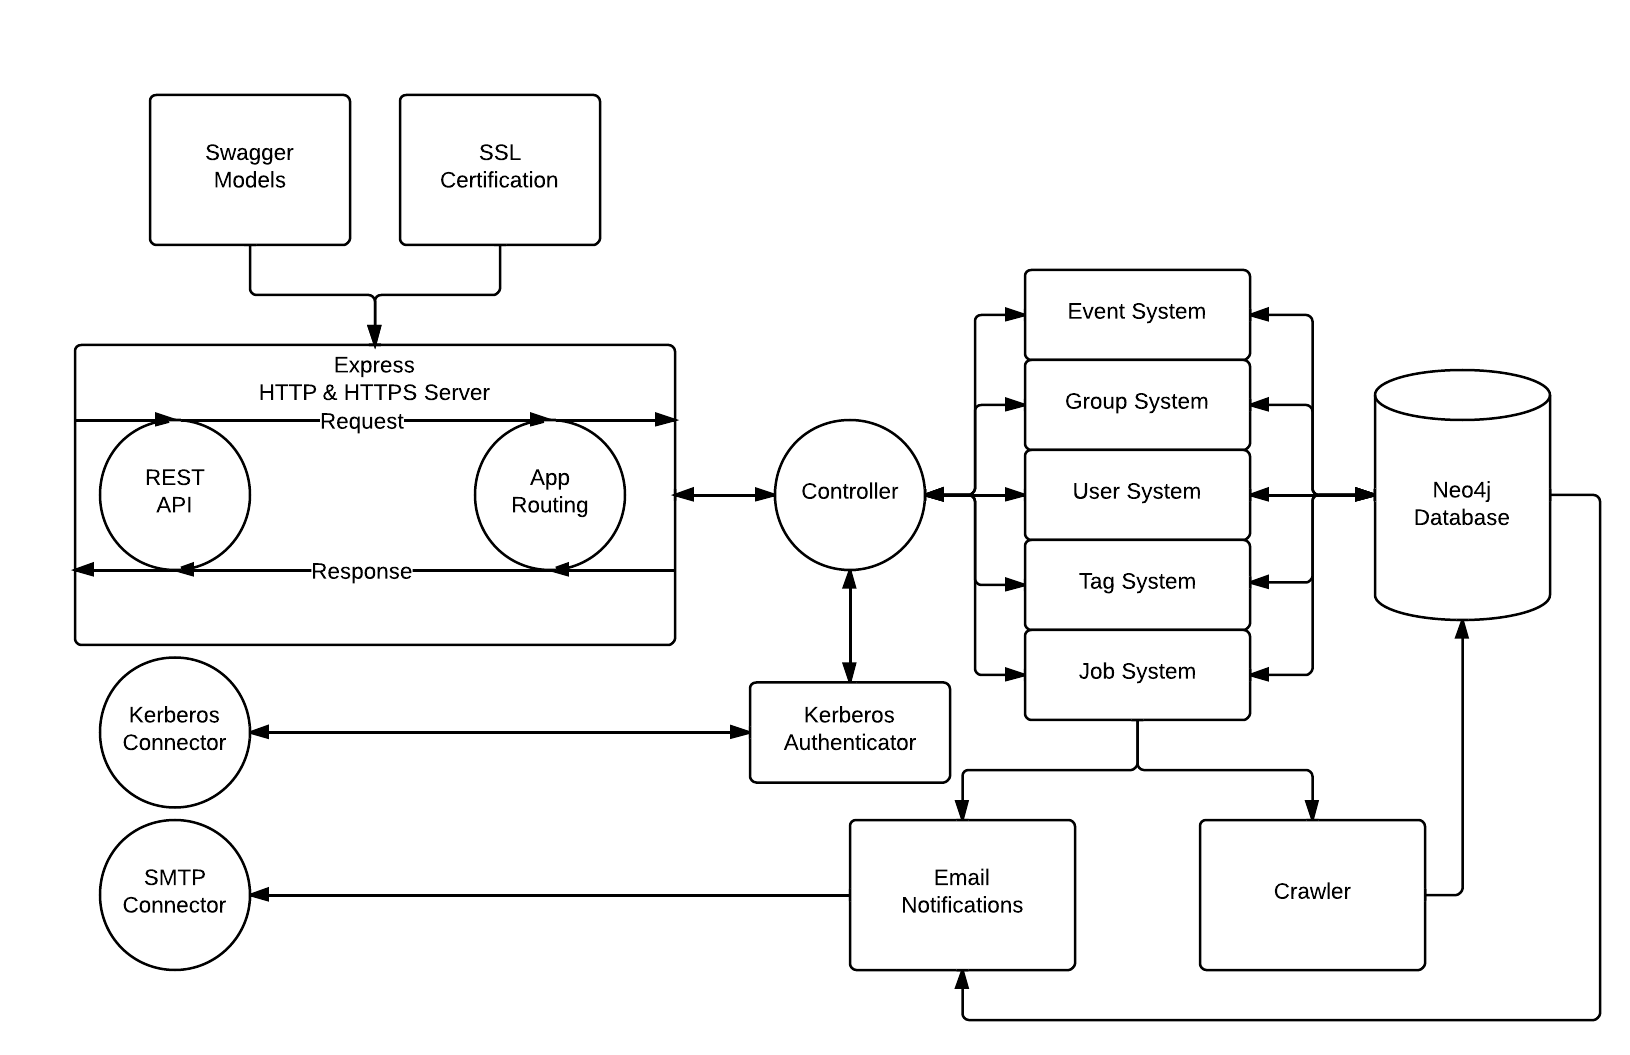
\includegraphics[scale=0.25]{./images/WebAppsBackendSystemDiagram.png}
}
\caption{\label{fig:backend-diagram} Backend System Design}
\end{figure}
\begin{figure}[H]
\centering
\fbox{
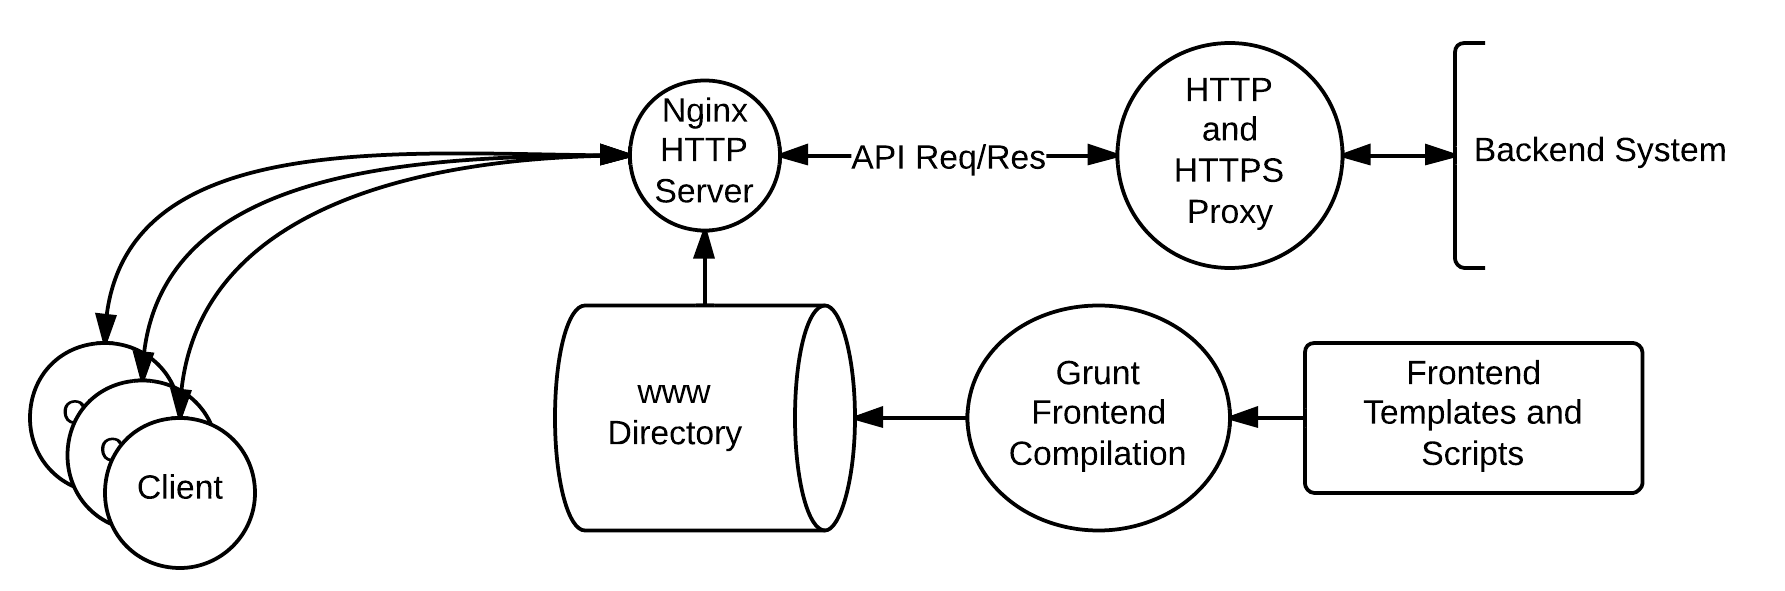
\includegraphics[scale=0.25]{./images/WebappsConnectionDiagram.png}
}
\caption{\label{fig:system-connectivity} System Connectivity}
\end{figure}


\subsection {Back End}

The backend is implemented with a Node.js server, allowing simple communciation and reusable code between backend and frontend. We split the project down into several categories, which we kept seperate from each other to minimize rigidity. Node.js is currently massively growing in popularity, and there are many useful libraries and frameworks which allow us to focus on writing application-specific code rather than the ``plumbing". Using Node.js also enabled us to develop both the front-end and back-end in CoffeeScript.

\subsubsection {API}
For the main API, we run express\footnote{\url{http://expressjs.com}}, a common package that has many plugins for enhanced ease of use in building web applications. On top of this we are running Swagger, a package built to ease documentation and design of RESTful interfaces. Swagger's major advantage is a one-command documentation/validator of the API, by running its validator and static documentation tool\footnote{https://github.com/wordnik/swagger-codegen} on the Node.js code itself. This allows us to perform basic unit testing to validate the UI whilst describing the UI for its documentation.
Swagger also provides an authentication callback, however we decided not to use this. We did this because the major limitation of its `validator' authentication callback is that it gets added to every HTTP request to authenticate it individually. We didn't want to do this, and instead split between HTTPS requests for logged in sessions, with user personalisation and extra permissions, and the public HTTP web application, which simply provides a simple way to view the upcoming calendar of public events. For authentication we used the Kerberos system, which ensured only college users could access the system.

\subsubsection {Crawler}
The crawler is used in order to synchronize out database with the information exposed by the already existing Imperial calendars which currently are the Union and the Imperial calendar.
The Union calendar does not expose the data in a machine readible format, so it was necessary to scrape the events directly from the HTML that the website provides.
In order to extract the relevant information we used the \textit{cheerio} framework. This is a framework that allows to operate on the HTML DOM in a similar fashion like using jQuery in a browser.

The events page from the Imperial homepage is syndicated via RSS. Using the node.js package \textit{feedparser} the fetched data was parsed into a JSON format. The JSON format was later converted into the relevant calendar format used by the Neo4j database.

\subsubsection{Notifications}
Email notifications are one of the services we provide for registered users. Each week, or other configured time, we collate the users subscriptions and send the upcoming events to them in an email. This is implemented via a connection to an SMTP server, a mining of the users subscribed events via a Cypher query, followed by a prettifying on the events and parsing into a HTML email via a templating engine.


\subsubsection{iCal}

By using the VObject from the \textit{jsDAV} library the events are easily converted and returned using the iCal format. The file contains the list of all of the events the user has subscribed to. This is the standard format used to display calendar events and is supported by online websites such as Outlook and Gmail and many desktop applications.

The calendar application fetches the iCal file from the given URL. In order to make users calendars private the server creates a random URL for each user. Thus only users that know a given URL can subscribe to the event. However the user can easily opt out from the URL as well as create a new one.

\subsubsection{Database}

The Neo4j database is a graph database that allows to quickly traverse the database.
Our database consists of a root node which has edges to nodes that are treated as `database tables'.
Creating a node for each table increases the search time. An alternative would be to create and index for each table node. This has the advantage of not having to specify a node that is treated as a root node.
The tables contain entries to relevant nodes (users, events, groups, etc.) that contain the relevant information saved as JSON data. Being stored in JSON format it is compatible with Node and the database can easily be upgraded. It is not necessary that all of the nodes in a given `table' have the same keys.

Nodes are connected by edges to define relationships like \textit{Friendship}, \textit{Following}, \textit{Member\_Of}.

\subsection{Problems or Limitations}

There are multiple problems to consider when designing an application as complex as this one.
Initially we split into back and front-end teams, but we found that developing the front-end was a much larger task for this application. This meant that we had to stop developing the back-end further in order to make the front-end as user friendly and as feature rich as possible.
The agile development allowed us to make the group reorganize themselves faster. Otherwise most likely the back-end would end up being very robust but for the end user the application would seem very simple.

On the front-end, we used a client-side package manager called "component". Though this library is well-designed, it is at a very early stage of development. As a result, its documentation is severely lacking in many places. This meant that we had to read the source in several instances to learn how certain things worked. Also, there were several issues with some of the library's plugins, for example the CoffeeScript compilation plugin was totally broken. As all the code is open source, MIT licensed and available on GitHub, we were able to fork the offending projects and fix the bugs ourselves. Some of the external libraries used also had to be fixed to work with "component", notably the natural language date parsing library "chrono". Again, forking the projects and fixing the problems ourselves was the easiest and fastest solution.

Another problem was initially that none of the team members had used the Neo4j database before. As such we had to learn its unique Cypher query language and try and work around any of the problems created by the queries, as it is very different from traditional SQL.

Secondly the application must respect information that is private to the users. In order to make sure that the user's passwords are not sent in plain text across the internet we decided to use SSL when establishing the login connection. SSL certificates are not free, however, so we self-signed our certificates. This means that on first use, web browsers will show a warning screen. Buying an SSL certificate would have alleviated this problem.

\subsection{Design Patterns}

The client-side architecture is based on the model-view-controller pattern. Backbone's naming conventions are slightly misleading. We found that the Backbone "View" class actually takes the place of a controller class in a standard MVC pattern: our Backbone "\textbf{V}iews" handle UI event actions, form validation, and keeping the model up to date. The "\textbf{v}iews" are actually the Jade templates, which generate the actual user-visible HTML 

\section {Legal Consideration}

For this project we've used sources from a wide variety of places. We've mostly been using the `npm' package manager for getting Node.js packages. In these packages, the default licence agreement is MIT, and we've checked this in each of the packages we've used. As such, there would be no major barriers to commercialising the product on that front.

On the legal issues for data use, we are using information crawled from Imperial College and Imperial College Union. Under Section 6 Part 2 of the College Data protection policy, it is required that personal data obtained and processed for a specific purpose must be only that which is sufficient to achieve that purpose, and held until that purpose is achieved, and must be obtained and processed `fairly'. It must be adequately protected, and if transferred to a country outside the EEA, must be ensured that that country can provide equivalent levels of protection. This information must also be registered using the departments central system.

\section {Conclusion}
We feel that our project is a huge step in the right direction to improving discovery of events happening across the Imperial campuses. We have started to collate information from multiple college-related sources (both the Imperial and Union calendars) and in the future we could implement software to perform Natural-Language Processing on other sources of information such as society newsletters to try and pull even more data into our system.

We have learned a lot of new technologies by undertaking this project, which has been a valuable experience, especially since they are very relevant in industry right now. However, if we were to do the project again, we'd think about using some more established projects in certain places, as the immaturity and instability of some of the newer libraries we used cost us a lot of time in trying to fix or work around small bugs.


\newpage
\section {Appendix}


\subsection {External Packages}
We used Node.js\footnote{\url{http://nodejs.org}} and CoffeeScript\footnote{\url{http://coffeescript.org}} on both the client and server sides. We also use nginx\footnote{\url{http://wiki.nginx.org/Main}} as the front-end server.

On the client-side, we used Component\footnote{\url{http://github.com/component/component}}, which is a client-side package manager. It bundles reusable JavaScript, CSS and HTML into `components', modules which can be reused in multiple places. 

We used several external client-side components:
\begin{itemize}
    \item \textbf{Backbone}\footnote{\url{http://github.com/solutionio/backbone}}: a minimal MVC library.
    \item \textbf{ListJS}\footnote{\url{http://github.com/cayasso/list}}: a JavaScript library which makes HTML lists sortable, filterable and searchable.
    \item \textbf{jQuery}\footnote{\url{http://github.com/component/jquery}}: a JavaScript library which adds many utilities including finding DOM elements by CSS-like selectors.
    \item \textbf{jade-runtime}\footnote{\url{http://github.com/monstercat/jade-runtime}}: the component used to evaluate Jade\footnote{Jade Template Engine: \url{http://jade-lang.com}} templates.
    \item \textbf{Underscore}\footnote{\url{http://github.com/component/underscore}}: a utility library used extensively with Backbone.
    \item \textbf{Moment}\footnote{\url{http://github.com/component/moment}}: a JavaScript date library making tasks such as formatting easier.
    \item \textbf{Chrono}\footnote{\url{http://github.com/lachenmayer/chrono}}: A natural language date parser in JavaScript.
    \item \textbf{Bacon.js}\footnote{\url{http://github.com/raimohanska/bacon.js}}: A natural language date parser in JavaScript.
    \item \textbf{Reset}:\footnote{\url{http://github.com/ianstormtaylor/reset}}: a CSS reset component.
\end{itemize}

On the back-end, we used the following Node.js modules:
\begin{itemize}
    \item \textbf{Express}: a library that creates a RESTful Http server
    \item \textbf{Swagger}: a library that creates an easy RESTful API
    \item \textbf{Cookie}:
    \item \textbf{jsDAV}\footnote{https://github.com/mikedeboer/jsDAV}: library that provides iCal support for node
    \item \textbf{node-feedparser}\footnote{https://github.com/danmactough/node-feedparser}: RSS parser for node
    \item \textbf{cheerio}\footnote{https://github.com/MatthewMueller/cheerio}: DOM parser for node
    \item \textbf{node-krb5}\footnote{https://github.com/qesuto/node-krb5}: kerberos authentication library
\end{itemize}

\newpage

\theendnotes


\end{document}

